
\documentclass[preprint,12pt]{elsarticle}

\usepackage[spanish]{babel}
\usepackage{amssymb}
\usepackage{graphicx}
\usepackage{lineno}
\usepackage[utf8]{inputenc}
\usepackage{url}
\usepackage{natbib} 
\usepackage{amsmath} 
\usepackage{amssymb} 

\begin{document}
	
	\begin{frontmatter} 

		\title{\huge MAPEO OBJETO RELACIONAL}
		
		\author{Estrella Palacios, Katherine Lizbeth              	(2016056193))}
		\author{Gonzales Cave, Angel Gabriel              	(2017057861))}
		\author{Huichi Contreras, Franklin Carlos         	(2016054948))} 
		\author{Huillca Umpiri, Willian Arturo             		(2015053793))} 
		\address{Escuela Profesional de Ingeniería de Sistemas}
		\address{Universidad Privada de Tacna}
		\address{Tacna, Perú}
		
%% ABSTRACT --------------------------------------------------------------------------------------------------------------------

		\begin{abstract}
		


		\end{abstract}

%% ----------------------------------------------------------------------------------------------------------------------------------

	\end{frontmatter}

%% RESUMEN ---------------------------------------------------------------------------------------------------------------------

\section{Resumen}



%% ----------------------------------------------------------------------------------------------------------------------------------


%% INTRODUCION ----------------------------------------------------------------------------------------------------------------

\section{Introducción} 
Varias áreas de aplicaciones para los sistemas de bases de datos se hallan limitadas por las restricciones del modelo de datos relacional. El modelo relacional orientado a objetos combina caracteristicas del modelo relacional y del modelo orientado a objetos. Este modelo proporciona un sistema de tipos de datos variado. Aplica la herencia a las relaciones, no sólo a los tipos . El modelo de datos relacional orientado a objetos permite una migración fácil desde las bases de datos relacionales.
El término base de datos orientada a objetos se utiliza para describir los sistemas de bases de datos que soportan el acceso directo a los datos desde lenguajes de programación orientados a objetos, sin necesidad de lenguajes de consultas relacionales como interfaz de las bases de datos.

%% ----------------------------------------------------------------------------------------------------------------------------------


%% MARCO TEÓRICO ------------------------------------------------------------------------------------------------------------

\section{Marco Teórico}

%% PRIMERA SUBSECCION 

\subsection {\textbf{Modelo de datos basado en objetos}}
El modelo de datos orientado a objetos se basa en el paradigma de los lenguajes de programación orientados a objetos, que actualmente se usa en gran medida. La herencia, la identidad de los objetos y la encapsulación , con métodos para ofrecer una interfaz para los objetos, están entre los conceptos principales de la programación orientada a objetos que han encontrado aplicación en el modelado de datos.

El modelo orientado a objetos puede considerarse una extensión del modelo E-R con los conceptos de encapsulación, métodos (funciones) e identidad de los objetos.

%%Ejemplo de cita
\cite{Gartner} 

\begin{itemize}
	\item x
	\item y
	\item z
\end{itemize}

\subsubsection{\textbf{A2}}

EDITAR\\

\subsubsection{\textbf{A3}}

EDITAR\\


%% SEGUNDA SUBSECCION

\subsection{\textbf{Bases de datos basadas en objetos}}
El primer obstáculo al que se enfrentan los programadores que usan el modelo relacional de datos es el limitado sistema de tipos soportado por el modelo relacional. El segundo obstáculo es la dificultad de acceso a los datos de la base de datos desde los programas escritos en lenguajes de programación como C++ o Java. La mera extensión del sistema de tipos soportado por las bases de datos no resulta suficiente para resolver completamente este problema.
El término lenguajes de programación persistentes hace referencia a las extensiones de los lenguajes de programación existentes que añaden persistencia y otras características de las bases de datos usando el sistema de tipos nativo del lenguaje de programación. El término sistemas de bases de datos orientadas a objetos se usa para hacer referencia a los sistemas de bases de datos que soportan sistemas de tipos orientados a objetos y permiten el acceso directo a los datos desde los lenguajes de programación orientados a objetos usando el sistema de tipos nativo del lenguaje.


\subsubsection{\textbf{Implementación de las características O-R}}

Los sistemas de bases de datos relacionales orientadas a objetos son básicamente extensiones de los sistemas de bases de datos relacionales ya existentes. Las modificaciones resultan claramente necesarias en muchos niveles del sistema de bases de datos. Sin embargo, para minimizar las modificaciones en el código del sistema de almacenamiento , los tipos de datos complejos soportados por los sistemas relacionales orientados a objetos se pueden traducir al sistema de tipos más sencillo de las bases de datos relacionales.

\subsubsection{\textbf{Lenguaje de programación persistentes}}
Los lenguajes de las bases de datos se diferencian de los lenguajes de programación tradicionales en que trabajan directamente con datos que son persistentes; es decir, los datos siguen existiendo una vez que el programa que los creó haya concluido. Las relaciones de las bases de datos y las tuplas de las relaciones son ejemplos de datos persistentes.
Los lenguajes de programación persistentes son lenguajes de programación extendidos con estructuras para el tratamiento de los datos persistentes. Los lenguajes de programación persistentes pueden distinguirse de los lenguajes con SQL incorporado, al menos, de dos maneras:

1. En los lenguajes incorporados el sistema de tipos del lenguaje anfitrión suele ser diferente del sistema de tipos del lenguaje para el tratamiento de los datos. Los programadores son responsables de las conversiones de tipos entre el lenguaje anfitrion y SQL. Hacer que los programadores lleven a cabo esta tarea presenta varios inconvenientes :
\begin{itemize}
	\item El código para la conversión entre objetos y tuplas opera fuera del sistema de tipos orientado a objetos y , por tanto tiene más posibilidades de presentar errores no detectados.
	\item La conversión en la base de datos entre el formato orientado a objetos y el formato relacional de las tuplas necesita gran cantidad de código.
\end{itemize}
2. Los programadores que usan lenguajes de consultas incorporados son responsables de la escritura de código explícito para la búsqueda en la memoria de los datos de la base de datos. Si se realizan actualizaciones , los programadores deben escribir explicitamente código para volver a guardar los datos actualizados en la base de datos.

\subsubsection{\textbf{Sistemas orientados a objetos y sistemas relacionales orientados a objetos}}

Los sistemas relacionales orientados a objetos se dirigen a simplificar la realización de los modelos de datos y de las consultas mediante el uso de tipos de datos complejos. Entre las aplicaciones habituales están el almacenamiento y la consulta de datos complejos, incluidos los datos multimedia.
Los lenguajes declarativos como SQL, sin embargo, imponen una reducción significativa del rendimiento a ciertos tipos de aplicaciones que se ejecutan principalmente en la memoria principal y realizan gran número de accesos a la base de datos. Los lenguajes de programación persistentes se dirigen a las aplicaciones de este tipo que tienen necesidad de un rendimiento elevado. Proporcionan acceso a los datos persistentes con poca sobrecarga y eliminan la necesidad de traducir los datos si hay que tratarlos con un lenguaje de programación. Sin embargo, son más susceptibles de deteriorar los datos debido a los errores de programación y no suelen disponer de gran capacidad de consulta. Entre las aplicaciones habituales están las bases de datos de CAD.

Los puntos fuertes de los diversos tipos de sistemas de bases de datos pueden resumirse de la manera siguiente:
\begin{itemize}
	\item Sistemas relacionales: tipos de datos sencillos, lenguajes de consultas potentes, protección elevada.
	\item Bases de datos orientadas a objetos basadas en lenguajes de programación persistentes: tipos de datos complejos, integración con los lenguajes de programación, elevado rendimiento.
	\item Sistemas relacionales orientados a objetos: tipos de datos complejos, lenguajes de consultas potentes, protección elevada.
\end{itemize}
%% Ejemplo de inclusión de imagen
\begin{figure}[htb]
	\begin{center}
		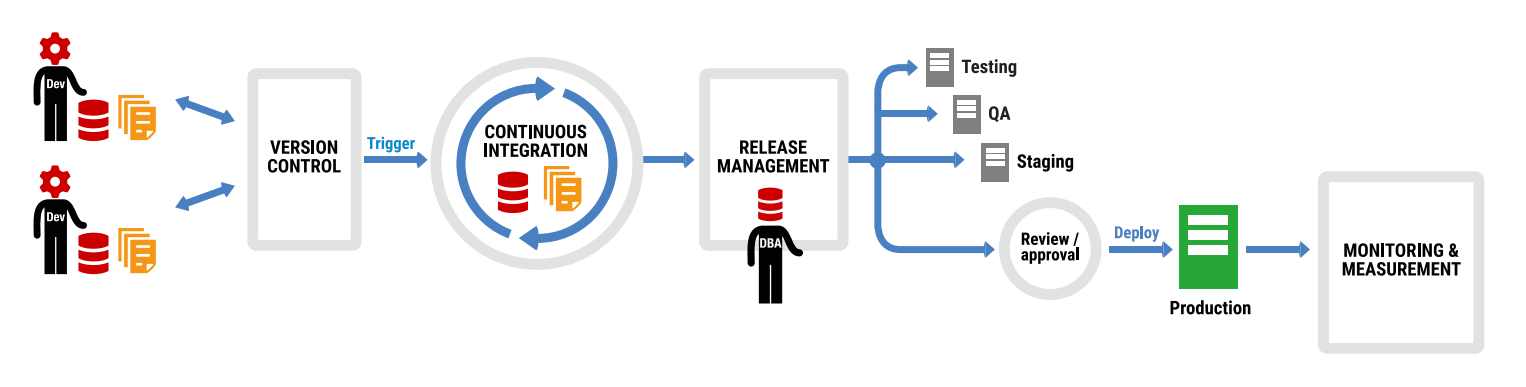
\includegraphics[width=14cm]{./IMAGENES/basededatos_1} 
		\caption{Incluyendo la base de datos en DevOps}
	\end{center}
\end{figure}

\subsubsection{\textbf{B2}}

EDITAR\\

%% TERCERA SUBSECCION
\subsection{\textbf{C}}

\subsubsection{\textbf{C1}}

EDITAR\\

\begin{itemize}

\item x
\item y
\item z

\end{itemize}
\subsubsection{\textbf{C2}}

EDITAR\\


%% ----------------------------------------------------------------------------------------------------------------------------------
 


%% ANÁLISIS ( APLICACIÓN ) ---------------------------------------------------------------------------------------------------

\section{Análisis}

\subsection{\textbf{Análisis 1}}
EDITAR\\

\subsection{\textbf{Análisis 2}}
EDITAR\\

\subsection{\textbf{Análisis 3}}
EDITAR\\

\subsection{\textbf{Análisis 4}}
EDITAR\\

%% ----------------------------------------------------------------------------------------------------------------------------------


%% CONCLUSIONES ---------------------------------------------------------------------------------------------------------------

\section{Conclusiones}

\begin{itemize}

\item Conclusion 1 : \\

\item Conclusion 2 : \\ 

\item Conclusion 3 : \\ 

\item Conclusion 4 : \\ 
\end{itemize}

%% ----------------------------------------------------------------------------------------------------------------------------------

%%  REFERENCIAS BIBLIOGRÁFICAS ------------------------------------------------------------------------------------------
	
	\newpage
	
	\bibliographystyle{apalike} 	%ESTILO
	\bibliography{BIBLIOGRAFIA}	 
	
	
\end{document}
